\section{Introduction}

The gig economy has revolutionized delivery services, yet most existing platforms prioritize customer convenience at the expense of courier well-being. \textbf{LiftDrop} addresses this imbalance by proposing a fairer, more efficient mobile application for last-mile deliveries.

\vspace{3mm}

\subsection{Motivation}

Gig economy platforms like Uber Eats, Glovo, and Bolt Food have become essential to urban logistics, offering convenience to customers and flexible work opportunities to couriers. However, these platforms exhibit systemic issues that disproportionately affect couriers and ultimately degrade overall service quality.

\subsection*{Key Issues in Existing Platforms}

\begin{itemize}
    \item \textbf{Unfair Order Assignment:} Many platforms use opaque algorithms that favor highly active or high-performing couriers, reinforcing inequality and disadvantaging new or less available workers.
    
    \item \textbf{Lack of Transparency:} Couriers typically receive minimal information about how their performance is evaluated, how earnings are calculated, or why specific orders are assigned. This opacity leads to distrust and confusion.
    
    \item \textbf{Safety Oversights:} Couriers are often routed through unsafe neighborhoods, especially at night, with little to no in-app risk alerts or mitigation strategies.
\end{itemize}

These challenges point to a systemic flaw: \textit{existing platforms are optimized for customer satisfaction rather than courier well-being.}

\bigskip

\textbf{LiftDrop} aims to correct this imbalance by embedding fairness, transparency, and safety at the core of its delivery model. By redesigning the order assignment logic, integrating safety monitoring, and promoting data transparency, LiftDrop introduces a more ethical and human-centered approach to delivery logistics.

\bigskip

\textbf{Key Objectives:}

\begin{itemize}
    \item Implement real-time order assignment based on proximity, traffic conditions, and fairness principles.
    \item Improve courier safety using neighborhood risk ratings and proactive alert systems.
    \item Develop a scalable Android application supported by two core APIs:
    \begin{itemize}
        \item \textbf{Courier API:} Manages orders and provides real-time updates via WebSockets.
        \item \textbf{Client Simulation API:} Simulates customer orders for testing and development purposes.
    \end{itemize}
\end{itemize}

\noindent
The figure below provides a high-level architectural view of the LiftDrop system. It illustrates the major components: the courier-facing mobile application, the client Web API for simulating orders, the backend server containing the business logic, the central database for persistent storage, and a geospatial API for calculating distances between couriers and delivery locations.

\bigskip

\begin{figure}[H]
    \centering
    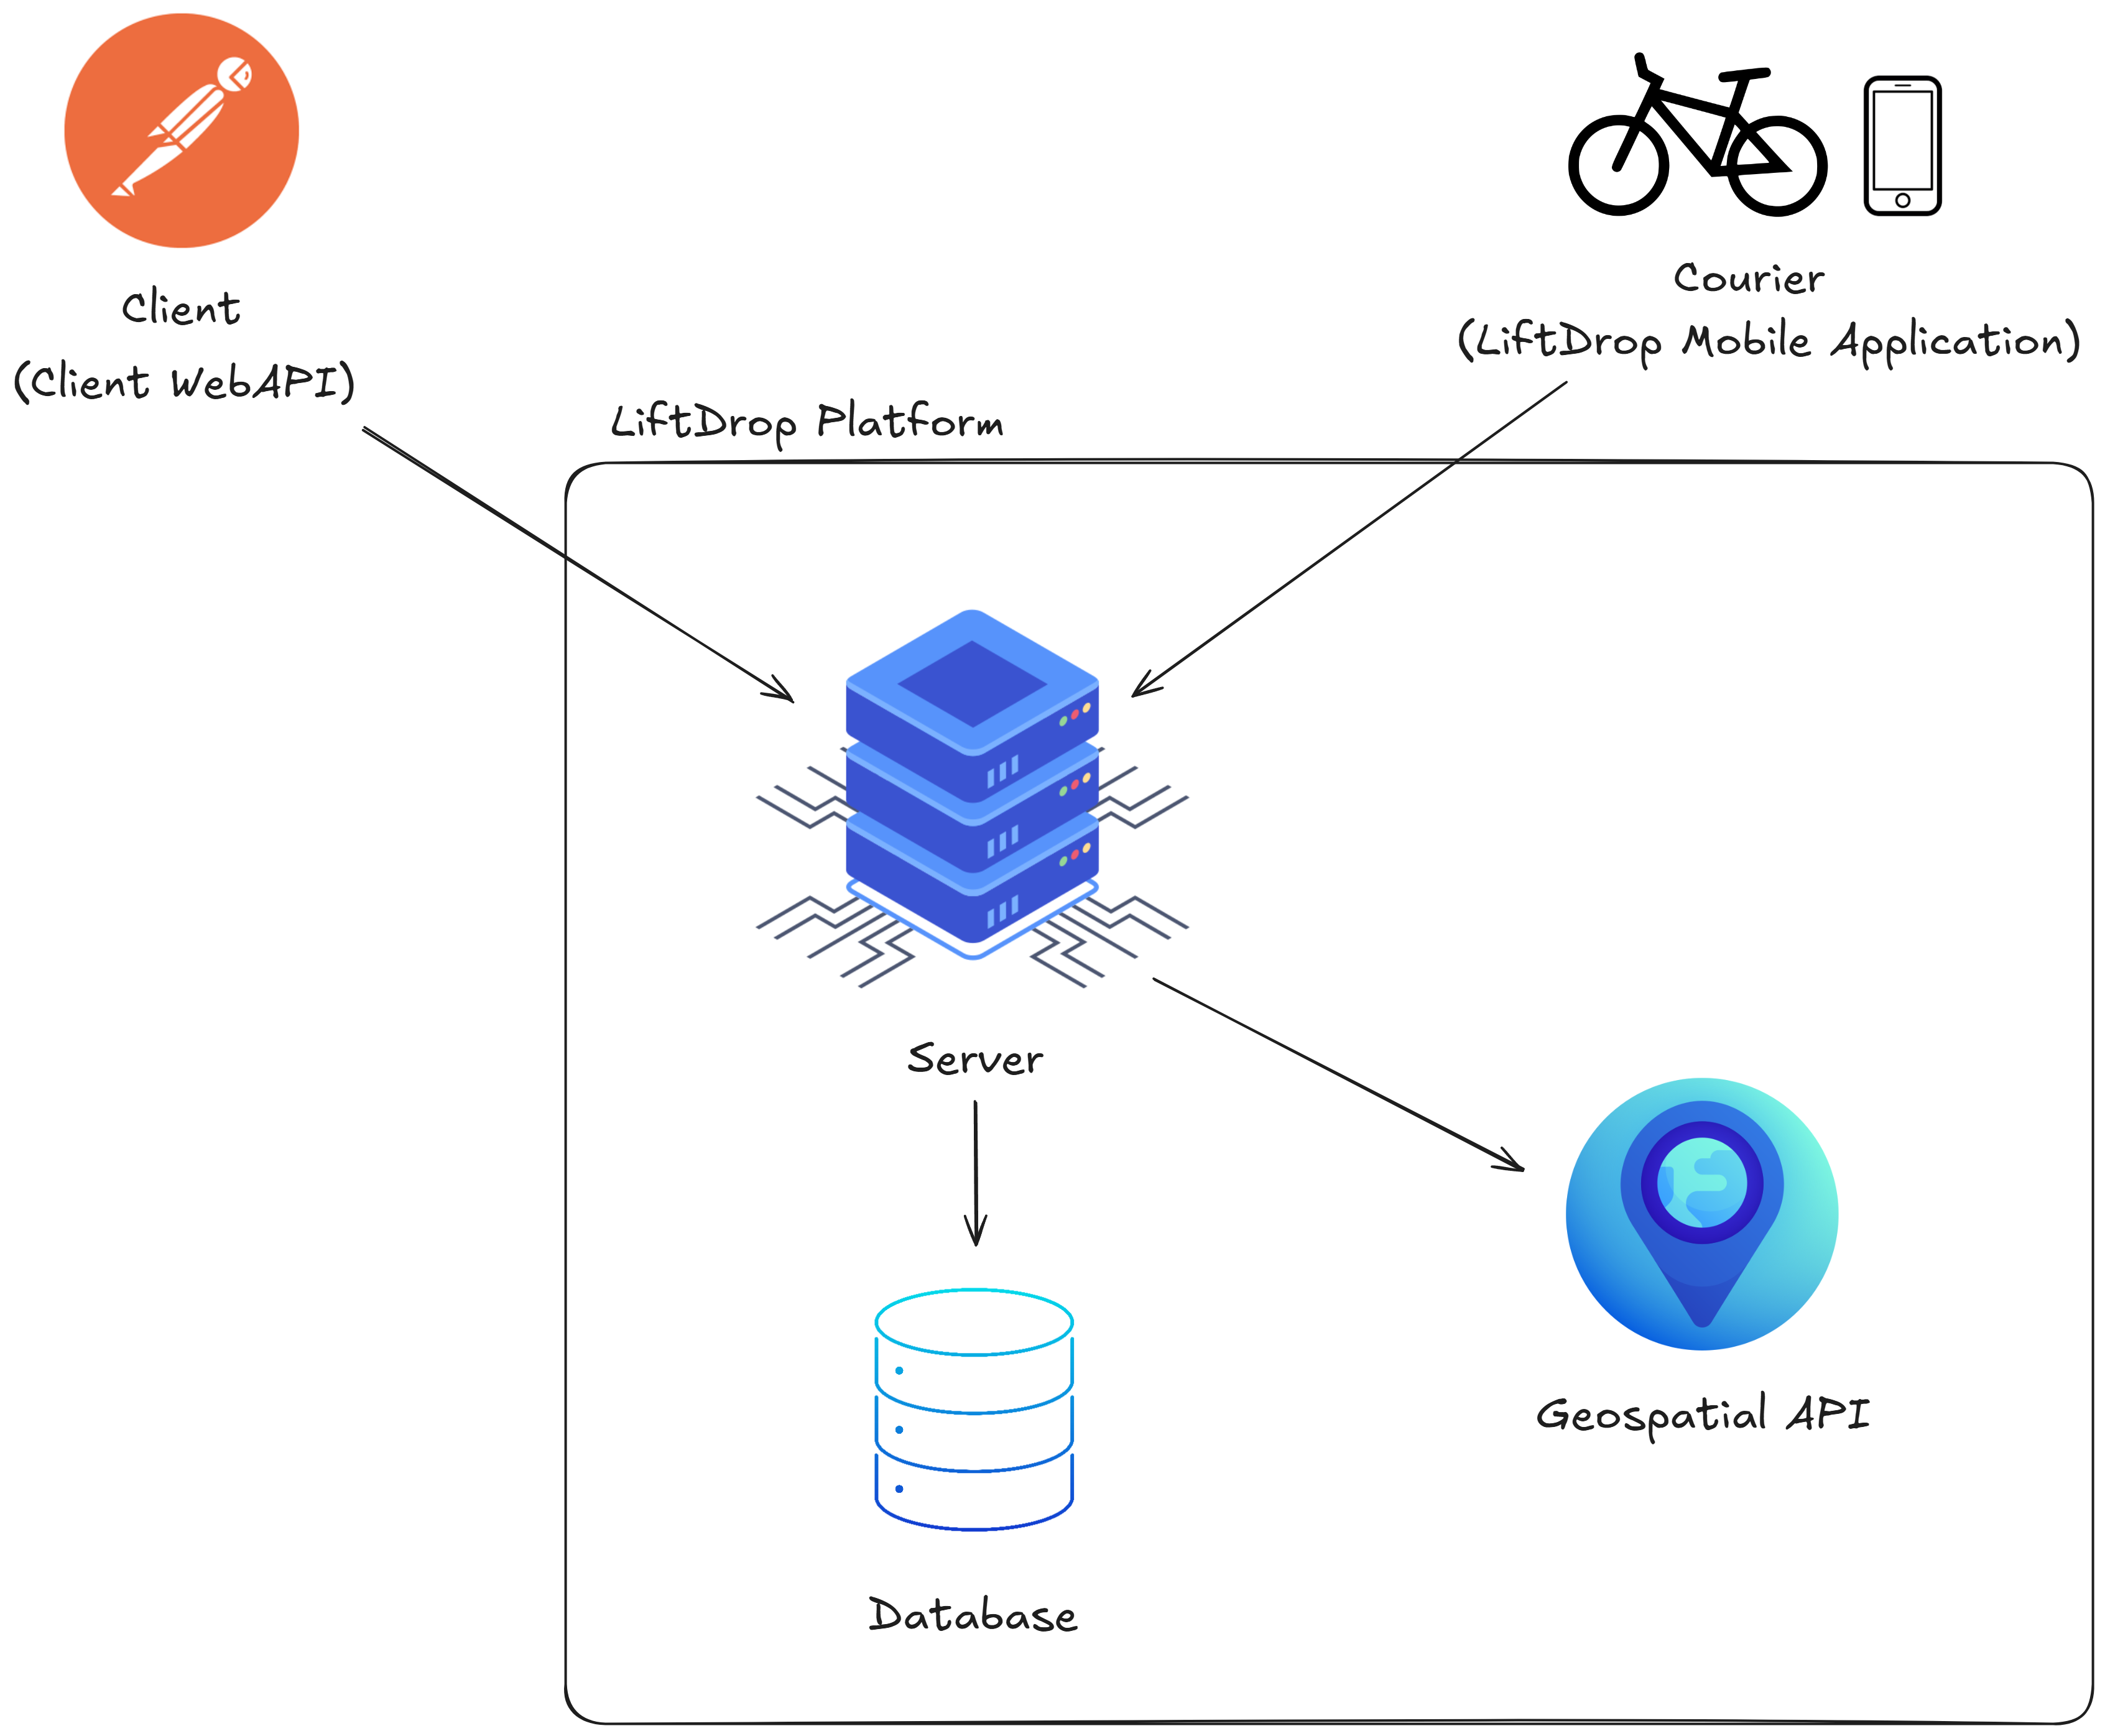
\includegraphics[width=0.55\textwidth]{images/LiftDrop_High_level_view.png}
    \caption{High-level overview of the LiftDrop system architecture}
    \label{fig:high-level-Overview}
\end{figure}

\noindent
\textbf{Figure \ref{fig:high-level-Overview}} summarizes the system's structure and component interactions without delving into implementation specifics.

\subsection{Requirements}

\subsection*{Functional Requirements}

The following features are essential for the success of the LiftDrop application:

\begin{itemize}
    \item Orders shall be assigned based on courier proximity, availability, and a fairness algorithm.
    \item Couriers shall receive visual safety ratings for neighborhoods within the mobile app.
    \item The Courier API shall provide real-time order status updates using WebSockets, ensuring timely communication.
\end{itemize}

\subsection{Organization}

This report is structured as follows: 
\begin{itemize}
    \item \textbf{Background Knowledge} provides an overview of the gig economy and logistics frameworks.
    \item \textbf{System Architecture} details the components and data flow within LiftDrop.
    \item \textbf{Interface Design} covers the user-facing aspects of the mobile application.
    \item \textbf{User Journey} demonstrates typical courier and client workflows.
    \item \textbf{Technical Implementation Details} discusses the development process and key technologies used.
\end{itemize}
